\subsection{Curricular Course Roles}
\label{sec:rolx}
Courses often play particular roles in their department, or across a
university. We already mentioned service courses that provide non
majors with a taste of the department's discipline. Personnel within a
department generally understand these roles. But department outsiders
do not possess such knowledge. Researchers such as education or
sociology scholars studying universities and colleges other than their
own have even less access to role information.

We illustrate here how {\em Via} can recover course ``roles.'' The
application of more sophisticated algorithms rooted in graph theory
allows {\em Via} users to detect both roles and communities within
course networks. To this end we applied a {\em RolX}
\cite{Henderson2012} analysis, which requires a graph representation of the enrollment data. Intuitively, the analysis attempts to identify sets of course
nodes across a graph that are similar in enrollment history, and
position in students' pathways. The algorithm then attempts to
identify families of such courses, analogously to how {\em k-means}
defines clusters. As with clustering, RolX does not provide semantics
for discovered clusters. Those must be provided by human
interpretation.

Concretely in terms of graph analysis concepts, we represent each
course as a six-dimensional vector of its:
\squishlist  % itemize with less space between the bullets.
  \item In-degree.
  \item Out-degree.
  \item Betweenness centrality: Sum of the fraction of all course pairs
    whose shortest enrollment paths pass through the course node.
  \item Closeness centrality: closeness to all other courses enrolled
    in after the course.
  \item Closeness centrality, reversed: closeness to all other courses
    enrolled in before the course.
  \item PageRank
\squishend
The {\em RolX} analysis clusters these vectors, resulting in three
course roles. 

Figure~\ref{fig:rolxOverview} shows a layout of courses by role.
\begin{figure}
    \centering
    \includegraphics{Figs/rolxOverviewCropped2PhotoshopCroppedDoctoredWhite.png}
    \caption{Overview of courses that fill one of three discovered
      {\em RolX} roles. Red: introductory; green: intermediate; blue:
      enrichment. (Elision and cropping to fit publication.)}
    \label{fig:rolxOverview}
\end{figure}
We manually---therefore subjectively---examined catalog descriptions
of courses in the three roles. The red courses are introductory into
their department's fields, such as {\em Introductory Fluids
  Engineering}. The green courses are intermediate offerings, which
would usually be taken by majors in the field. Another example from
this roles is {\em Computer Vision: From 3D Reconstruction to
  Recognition}. The final role, blue, comprises enrichment courses of
general interest and accessibility, and seminars.

In {\em Via} the roles turn into course attributes, by which we can
filter, color, and layout courses and
enrollments. Figure~\ref{fig:rolxIntroCourses} is the result of extracting
the subgraph in the center of Figure~\ref{fig:rolxOverview},
filtering to include only introductory-role courses, coloring course
nodes by discipline, and automatically having them laid out in
circles.
\begin{figure*}
    \centering
    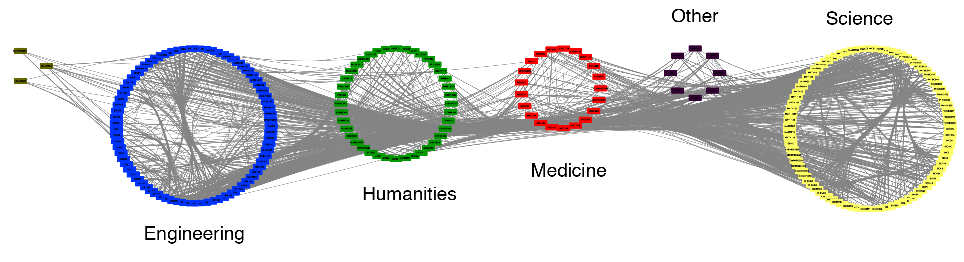
\includegraphics[width=\textwidth]{Figs/rolxIntroCoursesByDepartmentCropped.pdf}
    \caption{Introductory courses available in different disciplines.}
    \label{fig:rolxIntroCourses}
\end{figure*}
The task of finding introductory courses in the sciences now simply
involves clicking on any of the yellow nodes to see the course name,
or zooming in on the Science circle to see all the course name labels.

A final task that exploits roles is creation of an overview that shows
how many courses of each role the departments of the university
contribute to the curriculum. Figure~\ref{fig:rolxCircles} shows the
result.
\begin{figure}
    \centering
    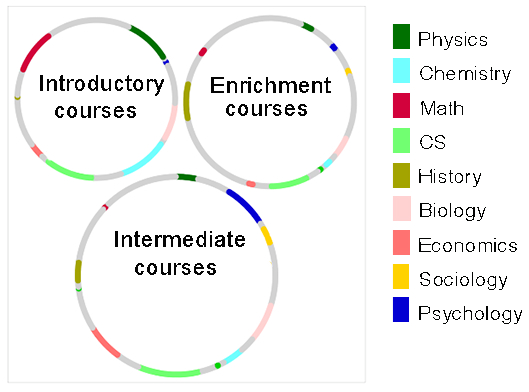
\includegraphics{Figs/rolxRingsCroppedLegendOutside.pdf}
    \caption{Which department offers courses in each of the three
      roles? (Legend created outside of tool.)
    }
    \label{fig:rolxCircles}
\end{figure}
Each circle's rim contains all courses that serve one role. The
circles were automatically constructed by requesting a circular layout
of all courses by the course role attribute. Courses of a particular
department were then selected by specifying that the names of courses
begin with, for example, {\em physics}. This action selected segments
of each role ring that was comprised of physics courses. The final
action was then to assign a color to those courses. The dark green
segments of the circles in the figure therefore indicate physics
courses.

